\section{Introduction}
\label{sec:introduction}

\begin{itemize}[leftmargin=0.6cm]
  \item A memory unit is a device to which binary information is transferred for storage and from which information is retrieved when needed for processing. A \textit{memory unit} is a \textit{collection of cells capable of storing a large quantity of binary information}.
  \item There are two types of memories that are used in digital systems: \textit{random-access memory} (RAM) and \textit{read-only memory} (ROM).
  \item The process of storing new information into memory is referred to as a memory \textit{write} operation. The process of transferring the stored information out of memory is referred to as a memory \textit{read} operation.
  \item RAM can perform \textit{both write and read} operations. ROM can \textit{perform only the read} operation.
  \item ROM is a \textbf{\textit{programmable logic device}} (\textit{PLD}).
  \item A RAM should be able to:
  \begin{itemize}[leftmargin=0.6cm]
    \item Store many words, one per address
    \item Read the word that was saved at a particular address
    \item Change the word that’s saved at a particular address
  \end{itemize}
\end{itemize}

Figure 1 shows the conventional and array logic symbols for a multiple input OR gate.
\begin{figure}[H]
  \centering
  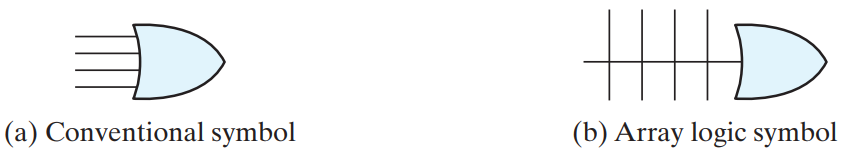
\includegraphics[width=\linewidth]{img/fig-7.1.png}
  \caption{Conventional and array logic diagrams for OR gate}
  \label{fig:7.1}
\end{figure}
